% Chapter Template

\chapter{Applications: Functional Linear Regression Modeling} % Main chapter title

\label{Chapter5} % Change X to a consecutive number; for referencing this chapter elsewhere, use \ref{ChapterX}

\lhead{Chapter 5. \emph{Applications: Functional Linear Regression Modeling}} % Change X to a consecutive number; this is for the header on each page - perhaps a shortened title

%----------------------------------------------------------------------------------------
%	SECTION 1
%----------------------------------------------------------------------------------------

\section{Introduction}

Chapter \ref{Chapter4} discussed the different types of functional linear regression models as well as the different criteria that should be applied in order to estimate these models. In this chapter, the interest will be on \textit{Functional Linear Regression} models where both the response variable and the independent variables are functional as defined in section~\ref{Funct_2}. The dataset that will be used to illustrate the modelling of functional variables is the \texttt{Aemet} data used by \cite{fda.usc} in their \texttt{R}-package \texttt{fda.usc}. This dataset has the following features:
\begin{itemize}
\item 73 weather stations selected over the time period 1980-2009;
\item 365 points of averaged \textit{temperature} from 1980 to 2009 evaluated at each station;
\item 365 points of averaged \textit{wind speed} from 1980 to 2009 evaluated at each station;
\item 365 points of averaged \textit{log-precipitation} from 1980 to 2009 evaluated at each station.
\end{itemize} 
The exercise of this chapter will be to predict the functional behaviour of the Log-Precipitation knowing the functional behaviours of Temperature, and Wind Speed for each weather station. In this case the functional linear regression equation can be written as follows:
\begin{equation}\label{chap5_eq1}
Y^{*}_i(t) = \int_{\mathcal{T}} X^{*}_{i1}(s) \beta_{1}(s,t)\mathrm{d}s + \int_{\mathcal{T}} X^{*}_{i2}(s) \beta_{2}(s,t)\mathrm{d}s + \epsilon_i(t), \text{ } \forall s, t \in \mathcal{T} 
\end{equation}
where $Y^{*}_i(t)$ is the centered functional variable for Log-Precipitation for the $i^{th}$ station, $X^{*}_{i1}(s)$ and $X^{*}_{i2}(s)$ are the centered functional variables for Temperature and Wind Speed respectively for $i^{th}$ station, and $\mathcal{T} = \left\{0.5,1.5,\dots,364.5\right\}$.  Since \textit{Least Squares} and \textit{Maximum Likelihood} methods often result in unstable estimators, the \textit{regularization} method is used to estimate the functional linear model \citep{Matsui2009}.

%-----------------------------------
%	SECTION 2
%-----------------------------------
\section{Methodology}\label{methodoly}
The computation of functional variables require a clear outline of the steps involved in modeling the functional behaviour of the Temperature and Wind Speed, and consequently the values of the Log-Precipitation at any given time point. Computing the \textit{Functional Linear Regression} model~\eqref{chap5_eq1} are done as follows:
\begin{itemize}
\item[Step 1] Center the data by substracting the mean across all stations;
\item[Step 2] Compute the GCV, GIC, GBIC and mAIC matrices for each station to find optimal values for $K$ and $\lambda$;
\item[Step 3] Add all the values obtained from \textbf{Step 2} for each criterion to compute $\hat{K}$ and $\hat{\lambda}$ that work for all stations;
\item[Step 4] Compute the $\bm{C}$ matrix of coefficients for each independent variable and the $\bm{D}$ matrix for the response variable using equation~\eqref{solution_eqpen};
\item[Step 5] Compute the matrices $\bm{J}_{\phi}$ leading to compute $\bm{Z}$ as explained at the end of section~\ref{Funct_2};
\item[Step 6] Compute the GCV, GIC, GBIC and mAIC matrices for each station (response variable) to find optimal value for $\lambda$ for a fixed value of $K$ computed in \textbf{Step 2} as explained in section~\ref{model_crit4};
\item[Step 7] Add all the values obtained from \textbf{Step 6} for each criterion to compute the matrices $\hat{\bm{\Sigma}}$ and $\hat{\bm{\mathcal{B}}}$ using equations \eqref{betahat2} and \eqref{sigma_hat};
\item[Step 8] Compute $\hat{\bm{D}}$ using equation~\eqref{hat_flrm}.
\end{itemize}
\clearpage
The above steps are executed for each of the three basis functions, namely: \textit{Gaussian}, \textit{Fourier} and \textit{B-splines}. Note that when the basis functions are orthonormal (e.g. \textit{Fourier}, \textit{B-Splines}), $\bm{J}_{\phi} = \mathbb{I}_{K^x_m}$. Another relevant point to note is that since the functions are observed at equally spaced timestamps, the \textit{Gaussian} basis functions with \textit{B-Splines} method is used to capture the functional behaviour of variables under \textit{Gaussian basis functions}.\\ 
Choosing the set of values over which the optimal number of basis functions $K$ is found is critical to the analysis. For large values of $K$ (i.e. 365 daily observations over the year), the bias in estimating the smooth functions is small. But of course, the estimated functions are not smooth and therefore increase their variability. Reducing the variance implies looking for smaller values of $K$, but at the same time not too small to make the bias unacceptable.  \cite{olberd:ramsay} used $\hat{K} = 65$ to smooth the \texttt{Canadian Weather} data in order to economize on computer time when dealing with daily observations.  In other words, the ideal smooth curve modelling the weather data is made of 65 basis functions which combines on average one basis function for 5 consecutive days of the year. For the case of the \texttt{Aemet} data, finding the optimal $K$-value depends on the model criterion chosen. A search of the optimal number of basis functions is computed for values of $K$ ranging from 5 to 65. In any case, the influence of smoothing parameter helps in adjusting the smoothness of the curve computed.
\\
\\
Extensive \texttt{R}-codes had to be written to compute all the basis functions and all model criteria to fit all 73 weather stations. Because of the amount of information that had to be computed a large number of times, the use of parallel computing was necessary. Appendix~\ref{AppendixA} presents the functions that were written in order to make the long \texttt{R} scripts readable. Some of these \texttt{R} functions were written with the help of \textrm{Dr. Shuichi KAWANO}, they are listed below:
\begin{itemize}
\item \texttt{Gaussian\_bsplines};
\item \texttt{Gaussian\_kmeans};
\item \texttt{Pen\_Max\_Likelihood};
\item \texttt{gic\_fun};
\item \texttt{mAIC\_fun}.
\end{itemize}
The \texttt{R} scripts can be found in the supplementary materials for this dissertation.
\clearpage
Table~\ref{table:table_all_stations} shows the values the optimal values for $\hat{K}$ and $\hat{\lambda}$ that were found by computing each model criterion on the all 73 stations. From the Table, it is clear that the \textit{Generalized Information Criterion} yields the lowest number of basis functions overall, and the \textit{modified Akaike Information Criterion} yields the lowest value of the smoothing parameter $10^{-5}$. Also, \textit{Fourier Basis} tends to result in small values of $K$, especially for Wind Speed and Log-Precipitation.

\begin{table}[ht]
\caption[Overall $\hat{K}$-values and log${}_{10}(\hat{\lambda})$ values computed for all stations]{$\hat{K}$ values and log${}_{10}(\hat{\lambda})$ values computed for all weather stations} 
\centering % used for centering table
\begin{tabular}{||l|l|l|r|r||} % centered columns (4 columns)
\hline\hline %inserts double horizontal lines
& & & & \\[-2ex]
 Functional Variables  & Types of Basis Functions   & Model Criteria & $\hat{K}$ & log${}_{10}\hat{\lambda}$ \\ [0.5ex]
%heading
\hline\hline 
\multirow{\textbf{Temperature}} & \multirow{Gaussian}  & GCV            & 		     63                          & -3.1                          \\
                              &                            & GIC            & 5                            & -1.72                          \\
                              &                            & mAIC           & 63                          & -3.1                          \\
                              &                            & GBIC           & 63                          & -1.03                           \\
                              \cline{2-5}
                              & \multirow{Fourier}   & GCV            & 63                          & -5.17                          \\
                              &                            & GIC            & 5                            & -1.72                          \\
                              &                            & mAIC           & 65                          & -5.17                          \\
                              &                            & GBIC           & 5                          & -5.86                          \\
                              \cline{2-5}
                              & \multirow{B-Splines} & GCV            & 63                          & -1.03                          \\
                              &                            & GIC            & 5                            & -1.72                          \\
                              &                            & mAIC           & 63                          & -3.1                          \\
                              &                            & GBIC           & 63                          & -1.03                          \\
                              \hline
\multirow{\textbf{Wind Speed}}  & \multirow{Gaussian}  & GCV            & 63                          & -2.41                          \\
                              &                            & GIC            & 5                            & -1.72                          \\
                              &                            & mAIC           & 63                          & -1.72                          \\
                              &                            & GBIC           & 63                          & 1.03                            \\
                              \cline{2-5}
                              & \multirow{Fourier}   & GCV            & 34                          & -4.48                          \\
                                                            &                            & GIC            & 5                            & -1.03                          \\
                                                            &                            & mAIC           & 34                          & -4.48                          \\
                                                            &                            & GBIC           & 5                          & -5.17                          \\
                              \cline{2-5}
                              & \multirow{B-Splines} & GCV            & 63                          & -2.41                         \\
                              &                            & GIC            & 5                            & -1.72                          \\
                              &                            & mAIC           & 63                          & -2.41                          \\
                              &                            & GBIC           & 63                          & 0.345                            \\
                              \hline
\multirow{\textbf{Log-Precipitation}}  & \multirow{Gaussian}  & GCV            & 51                          & -0.345                          \\
                              &                            & GIC            & 5                            & -2.41                          \\
                              &                            & mAIC           & 48                          & -0.345                          \\
                              &                            & GBIC           & 63                          & 0.345                            \\
                              \cline{2-5}
                              & \multirow{Fourier}   & GCV            & 7                           & -5.17                          \\
                              &                            & GIC            & 7                          & -5.17                          \\
                              &                            & mAIC           & 7                          & -5.17                          \\
                              &                            & GBIC           & 5                          & -5.17                            \\
                              \cline{2-5}
                              & \multirow{B-Splines} & GCV            & 63                          & -0.345                         \\
                              &                            & GIC            & 5                            & -3.1                          \\
                              &                            & mAIC           & 65                          & -0.345                          \\
                              &                            & GBIC           & 63                          & 0.345                            \\ [0.25ex] % [1ex] adds vertical space
\hline %inserts single line
\end{tabular}
\label{table:table_all_stations} % is used to refer this table in the text
\end{table}
\clearpage

%-----------------------------------
%	SECTION 2
%-----------------------------------

\section{Gaussian Basis Functions}

The focus of this section is to model functional variables (independent variables and response variable) specified in equation~\eqref{chap5_eq1} using \textit{Gaussian Basis} functions with \textit{Penalized Maximum Likelihood} estimate to compute the optimal model parameters $\hat{\bm{\Sigma}}$ amd $\hat{\bm{\mathcal{B}}}$.

\subsection{Temperature}
Figure~\ref{fig:Temp_Gauss} depicts the fitted curves implemented on the observed Temperatures at \texttt{A CORUÑA} using the information from Table~\ref{table:table_all_stations}. For this specific scenario, the \textit{Generalized Information Criterion} results in $\hat{K} = 5$ and $\hat{\lambda} = 10^{-1.72}$. The top right corner of Figure~\ref{fig:Temp_Gauss} shows a very smooth curve (blue line) on top the raw data, which is a different story for the other model criteria.

\begin{figure}[th]
  %\centering
    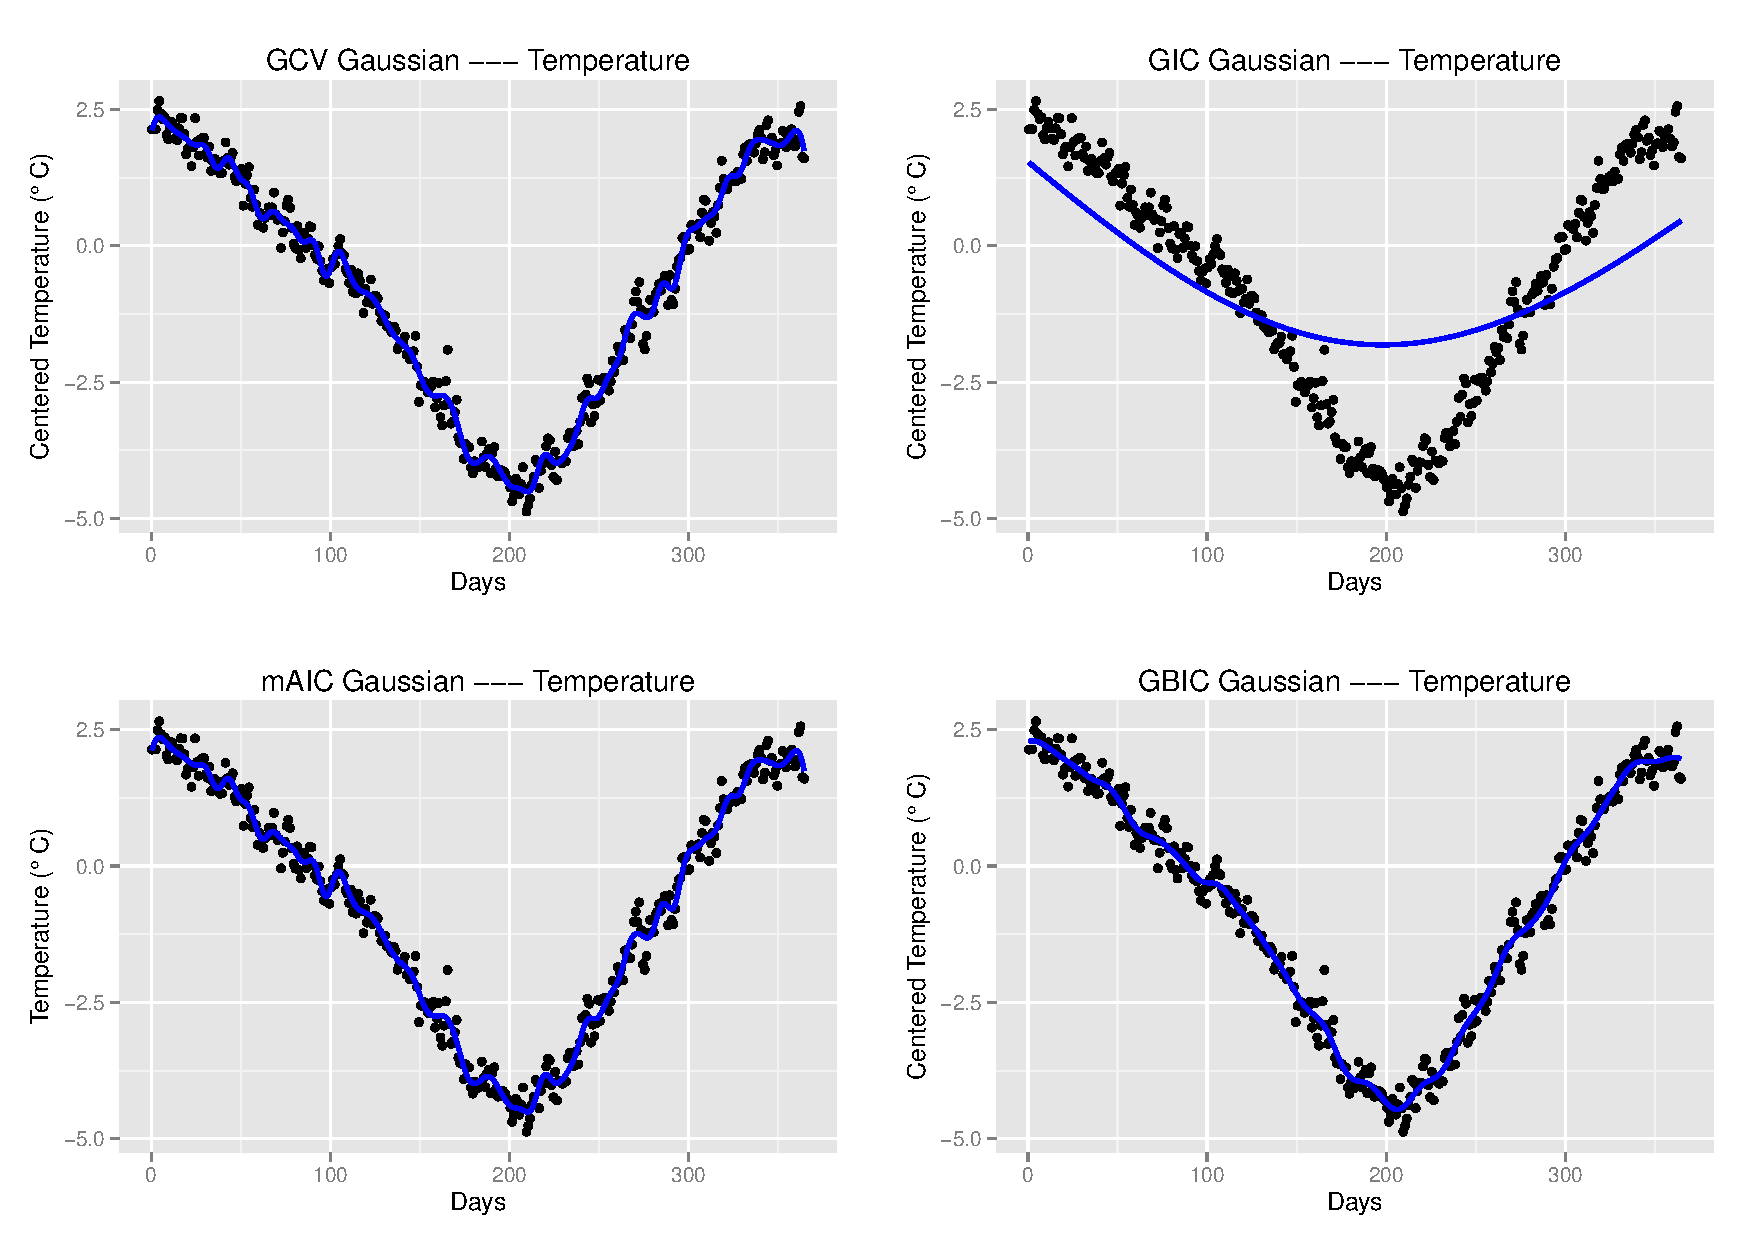
\includegraphics[height=12cm, width=1\textwidth]{Figures/Temp_Gauss_final.pdf}
  \caption[Fitting Temperature with \textit{Gaussian basis function} on \texttt{A CORUÑA} station]{\textbf{(a)} fitted curve using GCV; \textbf{(b)} fitted curve using GIC; \textbf{(c)} fitted curve using mAIC; \textbf{(d)} fitted curve using GBIC \\ on Temperatures in \texttt{A CORUÑA} }
  \label{fig:Temp_Gauss}
\end{figure}
\clearpage
\subsection{Wind Speed}
Figure~\ref{fig:wind_Gauss_2} depicts the fitted curves produced on the observed Wind Speed at \texttt{A CORUÑA} using the information from Table~\ref{table:table_all_stations}. For this specific scenario, the \textit{Generalized Information Criterion} results in $\hat{K} = 5$ and $\hat{\lambda} = 10^{-1.72}$, same as Temperature. The top right corner of Figure~\ref{fig:wind_Gauss_2} shows a very smooth curve (blue line) on top the raw data, which is a different story for the other model criteria.

\begin{figure}[th]
  %\centering
    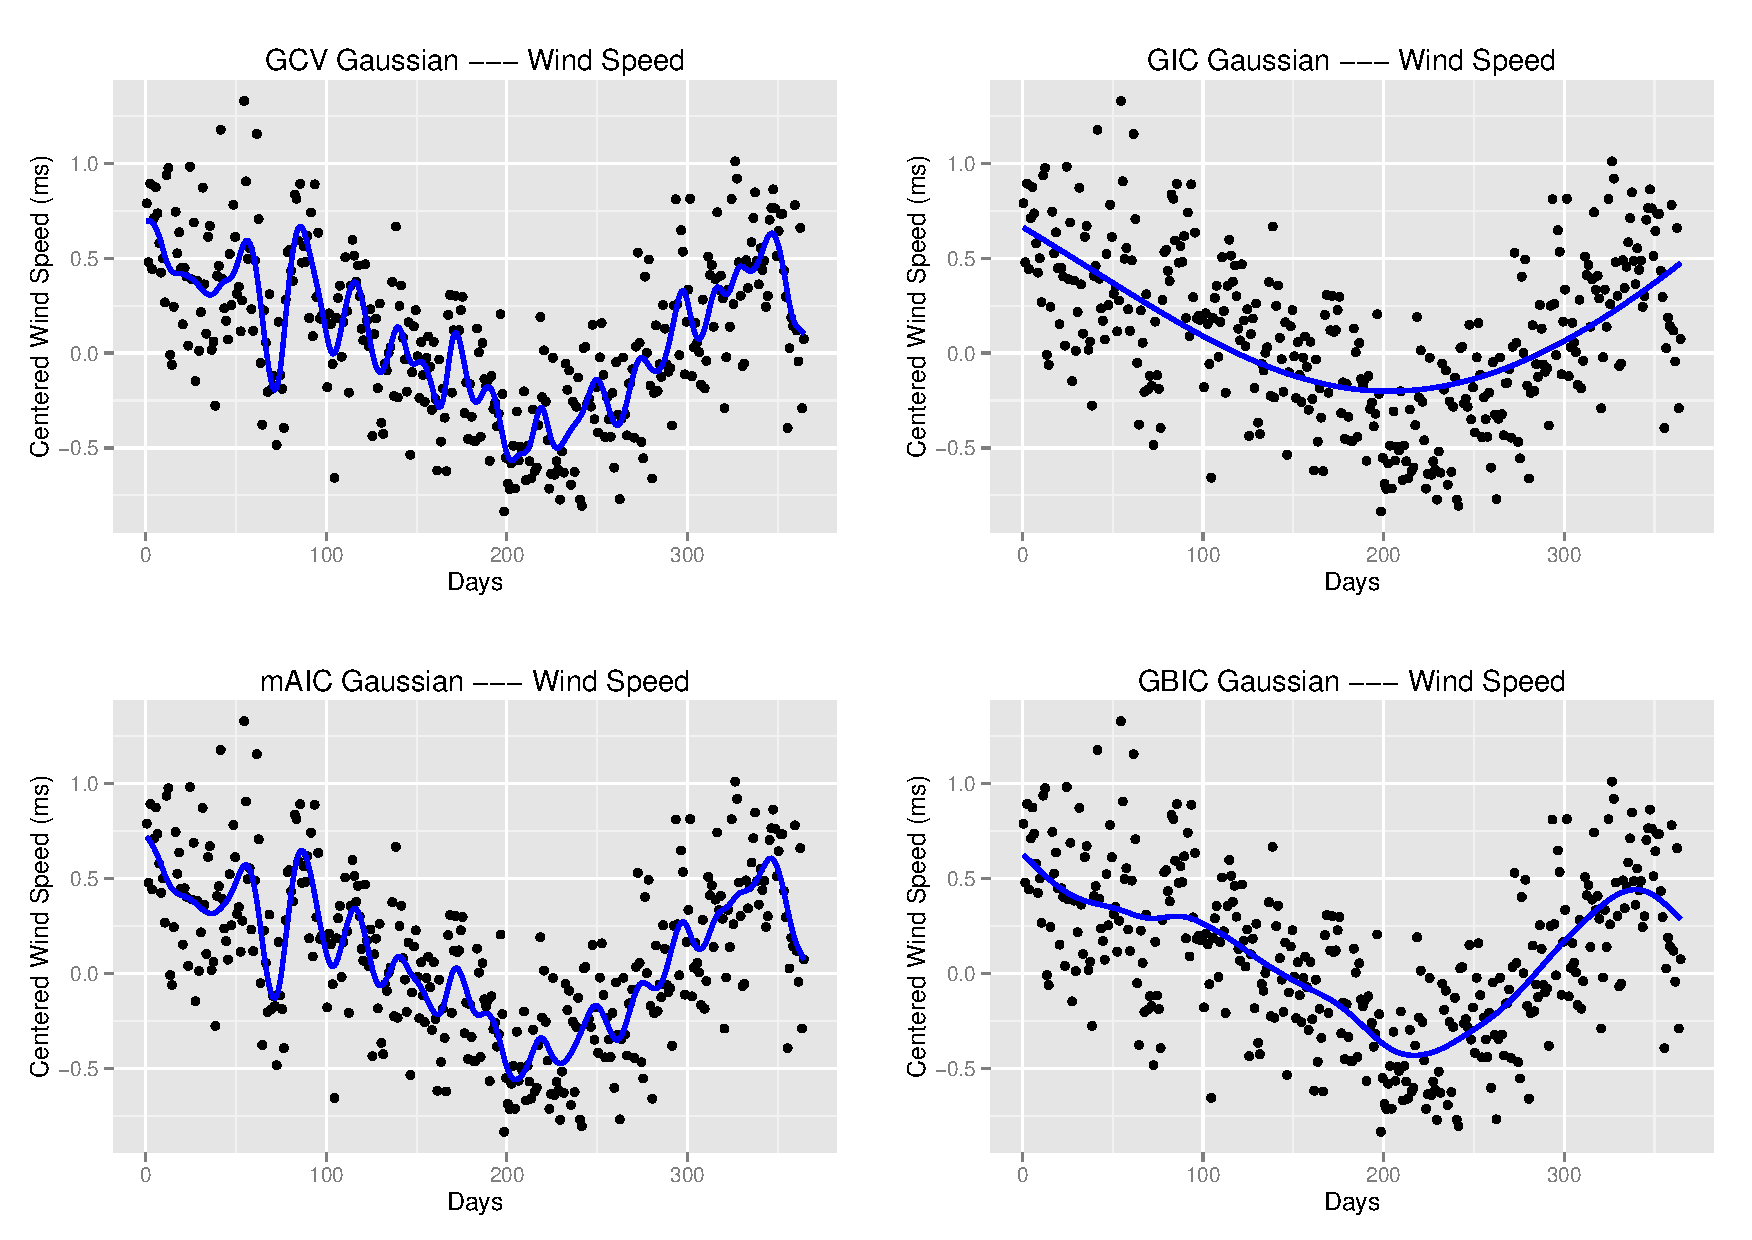
\includegraphics[height=12cm, width=1\textwidth]{Figures/Wind_Gauss_final.pdf}
  \caption[Fitting Wind Speed with \textit{Gaussian basis function} on \texttt{A CORUÑA} station]{\textbf{(a)} fitted curve using GCV; \textbf{(b)} fitted curve using GIC; \textbf{(c)} fitted curve using mAIC; \textbf{(d)} fitted curve using GBIC \\ on Wind Speed in \texttt{A CORUÑA}}
  \label{fig:wind_Gauss_2}
\end{figure}
\clearpage
\subsection{Log-Precipitation}
Computing the Log-Precipitation is done in two stages:\textbf{(1)} compute $\bm{D}$ then \textbf{(2)} compute $\bm{\hat{D}}$. Recall from Chapter~\ref{Chapter4} that $\bm{D}$ is a $N \times K_y$ matrix of coefficients with $N = 73$ and $K_y$ is the optimal number of basis functions computed following \textbf{Steps 1-4} from section~\ref{methodoly}. Their corresponding smoothing parameters $\hat{\lambda}$ are computed as well. The results are listed in Table~\ref{table:table_all_stations} of the Log-Precipitation using \textit{Gaussian Basis} functions. With all that information, it is possible to compute the matrices $\hat{\bm{\Sigma}}$ and $\hat{\bm{\mathcal{B}}}$ which yields to $\bm{\hat{D}}$. Because of hardware limitations, it is assumed that $\bm{\hat{D}}$ and $\bm{D}$ are of the same size and the optimization is only done on the smoothing parameters in order to get the optimal $\bm
{\Lambda}$. The use of equation~\eqref{hat_flrm} helps in calculating $\bm{\hat{D}}$.\\
Table~\ref{table:summary2} shows the optimal values $\text{log}_{10} (\hat{\lambda}_1)$ and $\text{log}_{10} (\hat{\lambda}_2)$ evaluated for all stations using each model criterion for a fixed the number of basis functions.
\begin{table}[ht]
\caption[Summary of the model selection on the Log-Precipitation using \textit{Gaussian basis functions}]{Summary of the model selection on the Log-Precipitation using \textit{Gaussian basis functions}}
\centering % used for centering table
\begin{tabular}{c @{\hspace{0.2cm}\vrule width 2pt\hspace{0.2cm}} c c c c } % centered columns (4 columns)
\hline %inserts double horizontal lines
\multicolumn{1}{c}{} & & & & \\[-2ex]
 \multicolumn{1}{c}{}& GCV & GIC & mAIC & GBIC \\ [0.5ex] % inserts table
%heading
\noalign{\hrule height 1pt} 
$\text{log}_{10} (\hat{\lambda}_1)$ & -3.41 & -1.42	& -3.72 & -2.33	\\
$\text{log}_{10} (\hat{\lambda}_2)$ & -2.1 & -1.92	& -2.1	& 0.33 \\
$\hat{K}$ & 51 & 5 & 48 & 63 \\
[0.25ex] % [1ex] adds vertical space
\hline  %inserts single line
\end{tabular}
\label{table:summary2} % is used to refer this table in the text
\end{table}

Figure~\ref{fig:logprec_Gauss} depicts the fitted curves produced on the observed Log-Precipitation at \texttt{A CORUÑA} using the information from Table~\ref{table:summary2}. The blue line represents the smooth curve computed using $\bm{D}$ and the red line represents the smooth curve derived from $\bm{\hat{D}}$. It can noted that the red lines has similar shape as the blue lines for each model criterion. Although the predicted curve for $\bm{\hat{D}}_{GIC}$ exhibits similar trend as the ones for $\bm{D}_{GIC}$, the fit is too smooth to be considered for further analysis. The top right corner plot confirms that statement. 

\newpage
\begin{landscape}
\thispagestyle{empty}
\begin{figure}[p]
  \centering
    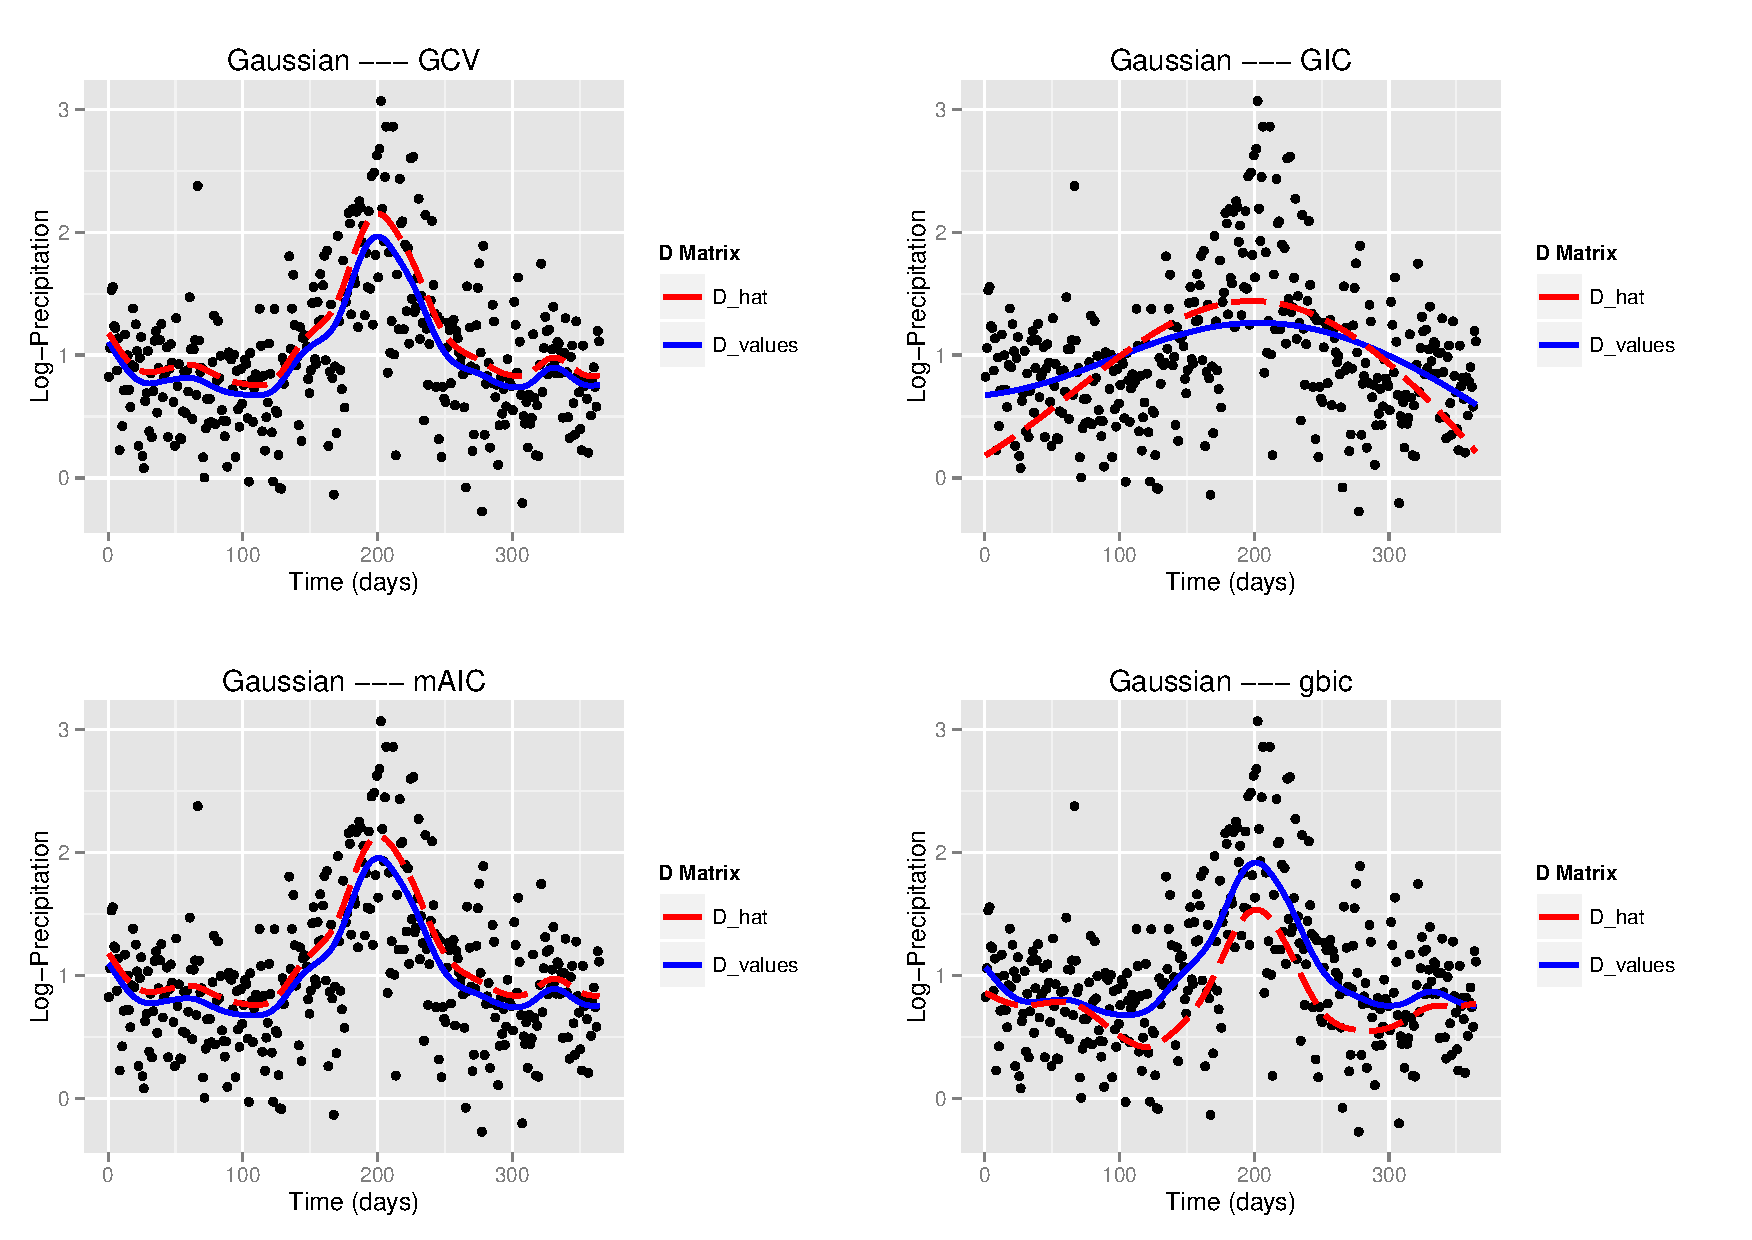
\includegraphics[height=15cm, width=1.7\textwidth]{Figures/D_hat_Gauss.pdf}
  \caption[Fitting Wind Speed with \textit{Gaussian basis function} on \texttt{A CORUÑA} station]{\textbf{(a)} fitted curve using GCV; \textbf{(b)} fitted curve using GIC; \textbf{(c)} fitted curve using mAIC; \textbf{(d)} fitted curve using GBIC \\ on Log-Precipitation in \texttt{A CORUÑA}}
  \label{fig:logprec_Gauss}
\end{figure}
\end{landscape}   
\newpage
%----------------------------------------------------------------------------------------
%	SECTION 2
%----------------------------------------------------------------------------------------

\section{Fourier Basis Functions}

The focus of this section is to model functional variables (independent variables and response variable) specified in equation~\eqref{chap5_eq1} using \textit{Fourier Basis} functions with \textit{Penalized Maximum Likelihood} estimate to compute the optimal model parameters $\hat{\bm{\Sigma}}$ amd $\hat{\bm{\mathcal{B}}}$.

\subsection{Temperature}
Figure~\ref{fig:Temp_fourier} depicts the fitted curves produced on the observed Temperature at \texttt{A CORUÑA} using the information from Table~\ref{table:table_all_stations}. For this case, once again the \textit{Generalized Information Criterion} has elected small values for $K$ and $\lambda$, smaller than the other model criteria. Clearly the small number of basis functions, has an important impact on the shape of the curve.

\begin{figure}[th]
  %\centering
    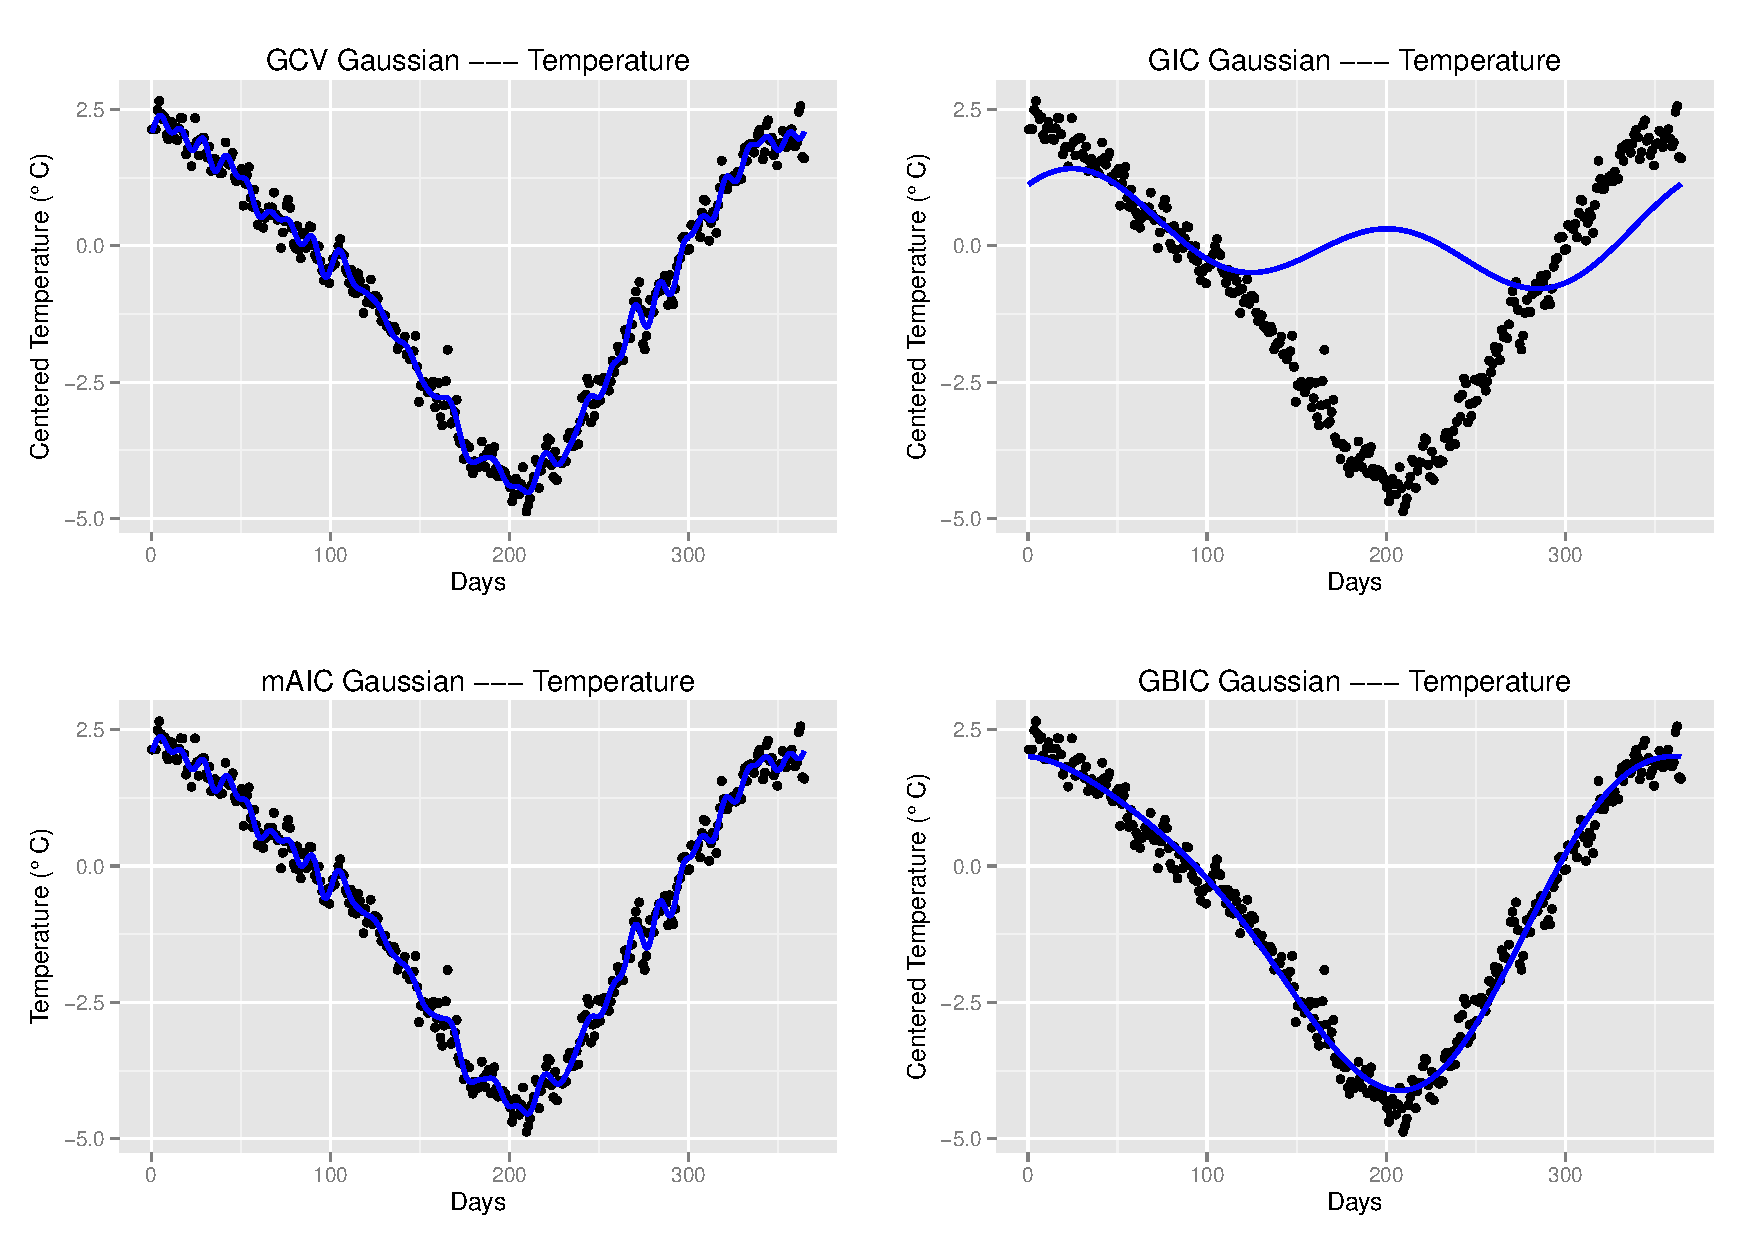
\includegraphics[height=12cm, width=1\textwidth]{Figures/Temp_fourier_plot.pdf}
  \caption[Fitting Temperature with \textit{Fourier basis function} on \texttt{A CORUÑA} station]{\textbf{(a)} fitted curve using GCV; \textbf{(b)} fitted curve using GIC; \textbf{(c)} fitted curve using mAIC; \textbf{(d)} fitted curve using GBIC \\ on Temperatures in \texttt{A CORUÑA} }
  \label{fig:Temp_fourier}
\end{figure}
\clearpage
\subsection{Wind Speed}
Figure~\ref{fig:Wind_fourier_plot} depicts the fitted curves produced on the observed Wind Speed at \texttt{A CORUÑA} using the information from Table~\ref{table:table_all_stations}. For this case, the \textit{Generalized Information Criterion} and the \textit{Generalized Bayesian Information Criterion} result in small $\hat{K}$ and small $\hat{\lambda}$. The top and bottow right hand side of Figure~\ref{fig:Wind_fourier_plot} show very smooth curves (blue line).
\begin{figure}[th]
  %\centering
    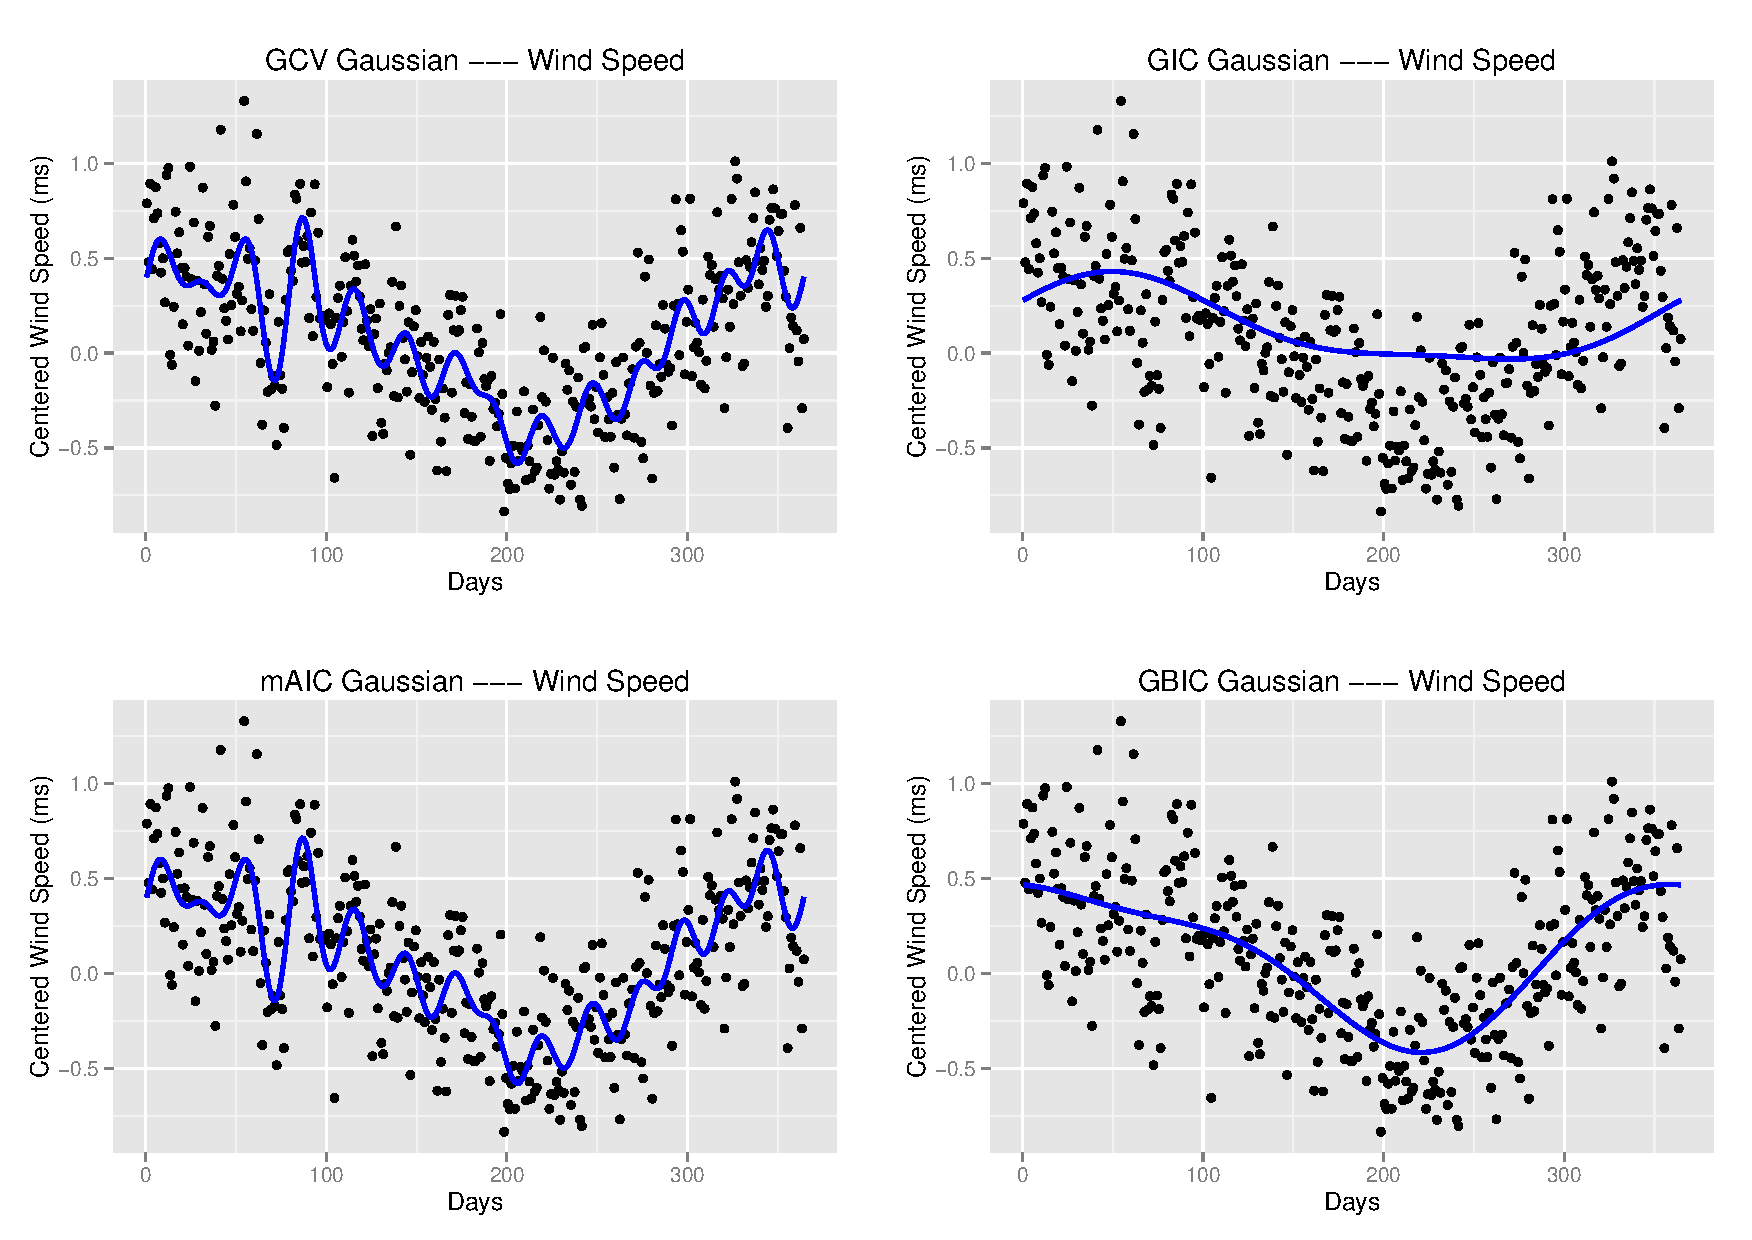
\includegraphics[height=12cm, width=1\textwidth]{Figures/Wind_fourier_plot.pdf}
  \caption[Fitting Wind Speed with \textit{Fourier basis function} on \texttt{A CORUÑA} station]{\textbf{(a)} fitted curve using GCV; \textbf{(b)} fitted curve using GIC; \textbf{(c)} fitted curve using mAIC; \textbf{(d)} fitted curve using GBIC \\ on Wind Speed in \texttt{A CORUÑA}}
  \label{fig:Wind_fourier_plot}
\end{figure}
\clearpage
\subsection{Log-Precipitation}
Table~\ref{table:summary4} shows the optimal values $\text{log}_{10} (\hat{\lambda}_1)$ and $\text{log}_{10} (\hat{\lambda}_2)$ evaluated for all stations using each model criterion for a fixed the number of basis functions. Note that the optimal number of basis functions is quite small for all basis functions and $\text{log}_{10} (\hat{\lambda})$ values are all negatives.
\begin{table}[ht]
\caption[Summary of the model selection on the Log-Precipitation using \textit{Fourier basis functions}]{Summary of the model selection on the Log-Precipitation using \textit{Fourier basis functions}}
\centering % used for centering table
\begin{tabular}{c @{\hspace{0.2cm}\vrule width 2pt\hspace{0.2cm}} c c c c } % centered columns (4 columns)
\hline %inserts double horizontal lines
\multicolumn{1}{c}{} & & & & \\[-2ex]
 \multicolumn{1}{c}{}& GCV & GIC & mAIC & GBIC \\ [0.5ex] % inserts table
%heading
\noalign{\hrule height 1pt} 
$\text{log}_{10} (\hat{\lambda}_1)$ & -4.83 & -1.52	& -5.25 & -5.17	\\
$\text{log}_{10} (\hat{\lambda}_2)$ & -3.92 & -1.25	& -4.21	& -5.17 \\
$\hat{K}$ & 7 & 7 & 7 & 5 \\
[0.25ex] % [1ex] adds vertical space
\hline  %inserts single line
\end{tabular}
\label{table:summary3} % is used to refer this table in the text
\end{table}

Figure~\ref{fig:logprec_fourier} depicts the fitted curves produced on the observed Log-Precipitation at \texttt{A CORUÑA} using the information from Table~\ref{table:summary3}. The blue line represents the smooth curve computed using $\bm{D}$ and the red line represents the smooth curve derived from $\bm{\hat{D}}$.

\newpage
\begin{landscape}
\thispagestyle{empty}
\begin{figure}[p]
  \centering
    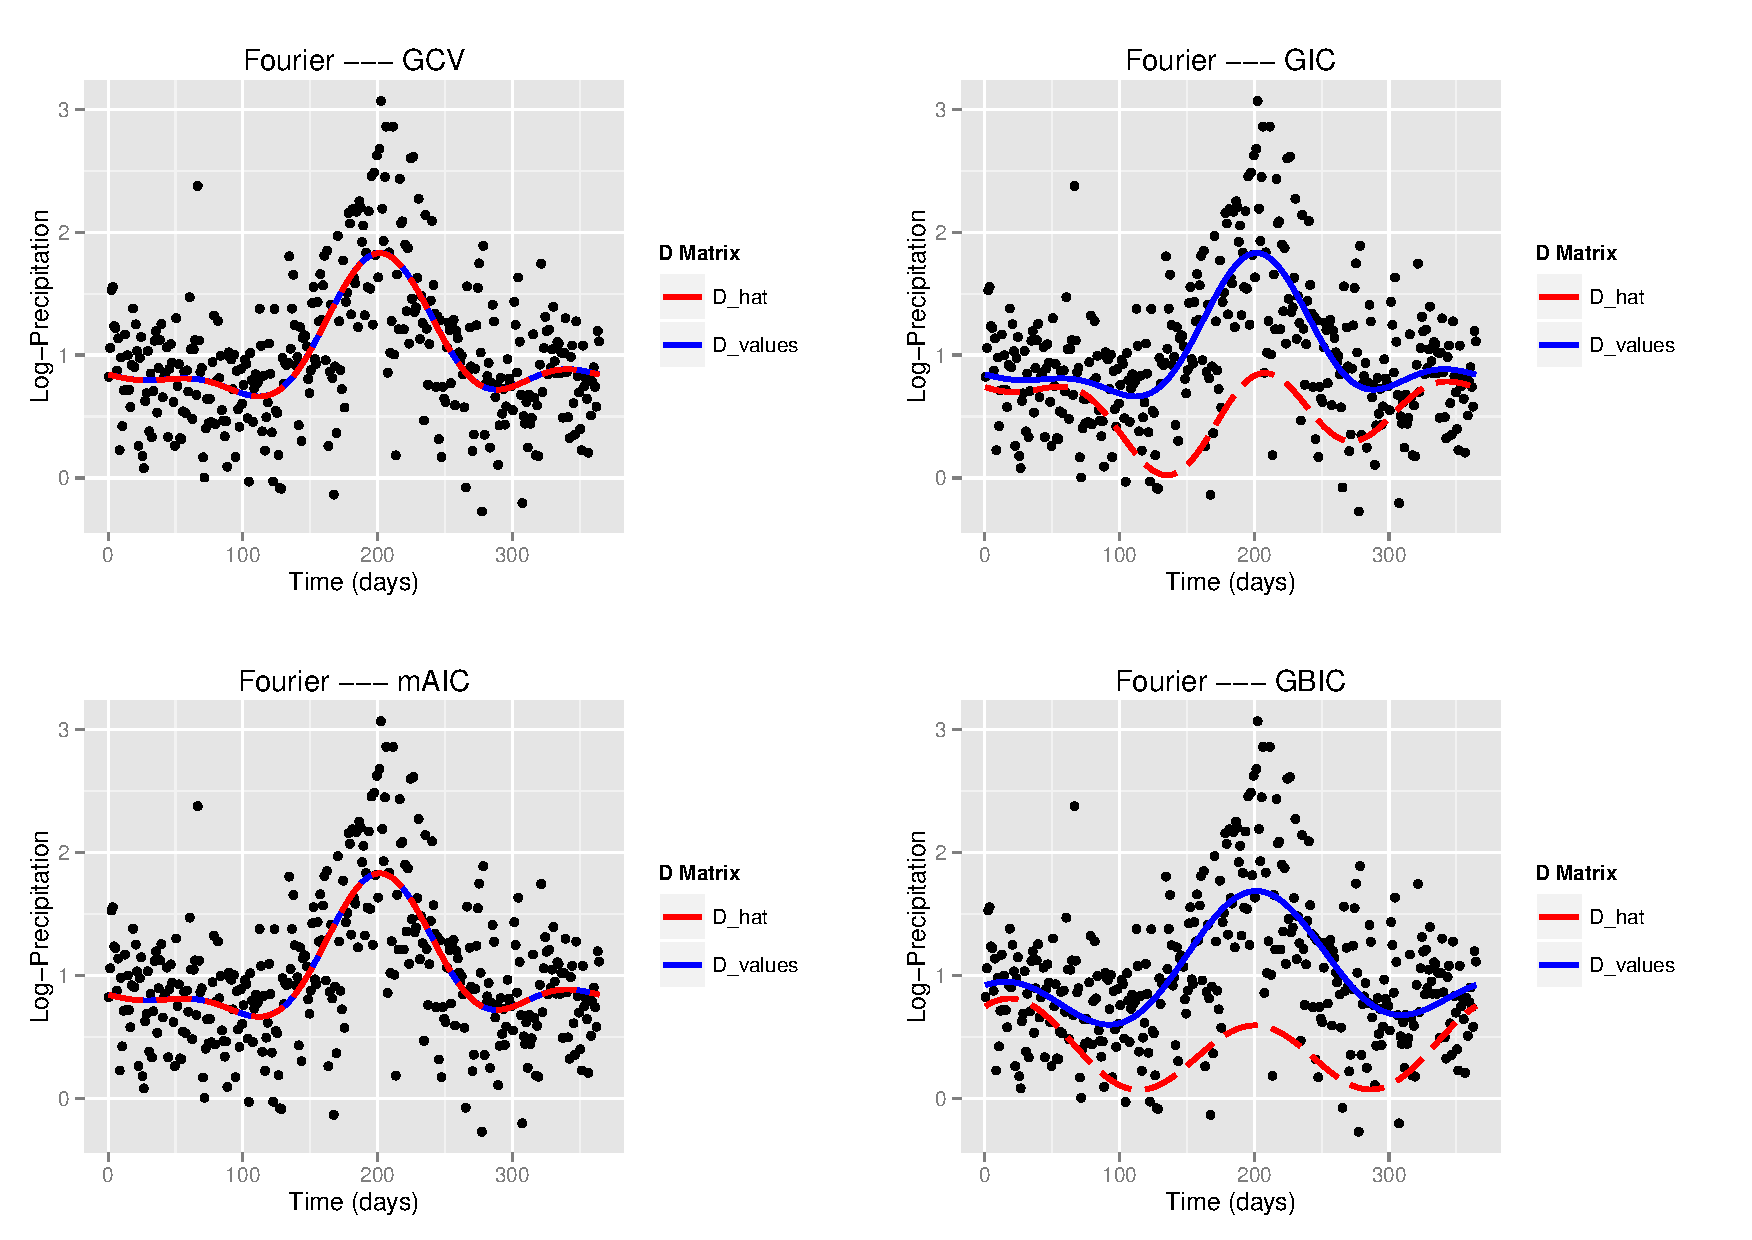
\includegraphics[height=15cm, width=1.7\textwidth]{Figures/D_hat_Fourier.pdf}
  \caption[Fitting Wind Speed with \textit{B-Splines basis function} on \texttt{A CORUÑA} station]{\textbf{(a)} fitted curve using GCV; \textbf{(b)} fitted curve using GIC; \textbf{(c)} fitted curve using mAIC; \textbf{(d)} fitted curve using GBIC \\ on Log-Precipitation in \texttt{A CORUÑA}}
  \label{fig:logprec_fourier}
\end{figure}
\end{landscape}   
\newpage

\section{B-Splines Basis Functions}
In this section the modeling is done using \textit{B-Splines basis functions} with \textit{Penalized Maximum Likelihood} estimate to calculate the functional the linear regression model (see equation~\eqref{chap5_eq1}). 

\subsection{Temperature}
Figure~\ref{fig:Temp_bsplines} shows the fitted curves produced on the observed Temperature at \texttt{A CORUÑA} using the information from Table~\ref{table:table_all_stations}. For this case, once again the \textit{Generalized Information Criterion} has elected small values for $K$ and $\lambda$, smaller than the other model criteria. Clearly the small number of basis functions, has an important impact on the shape of the curve.


\begin{figure}[th]
  %\centering
    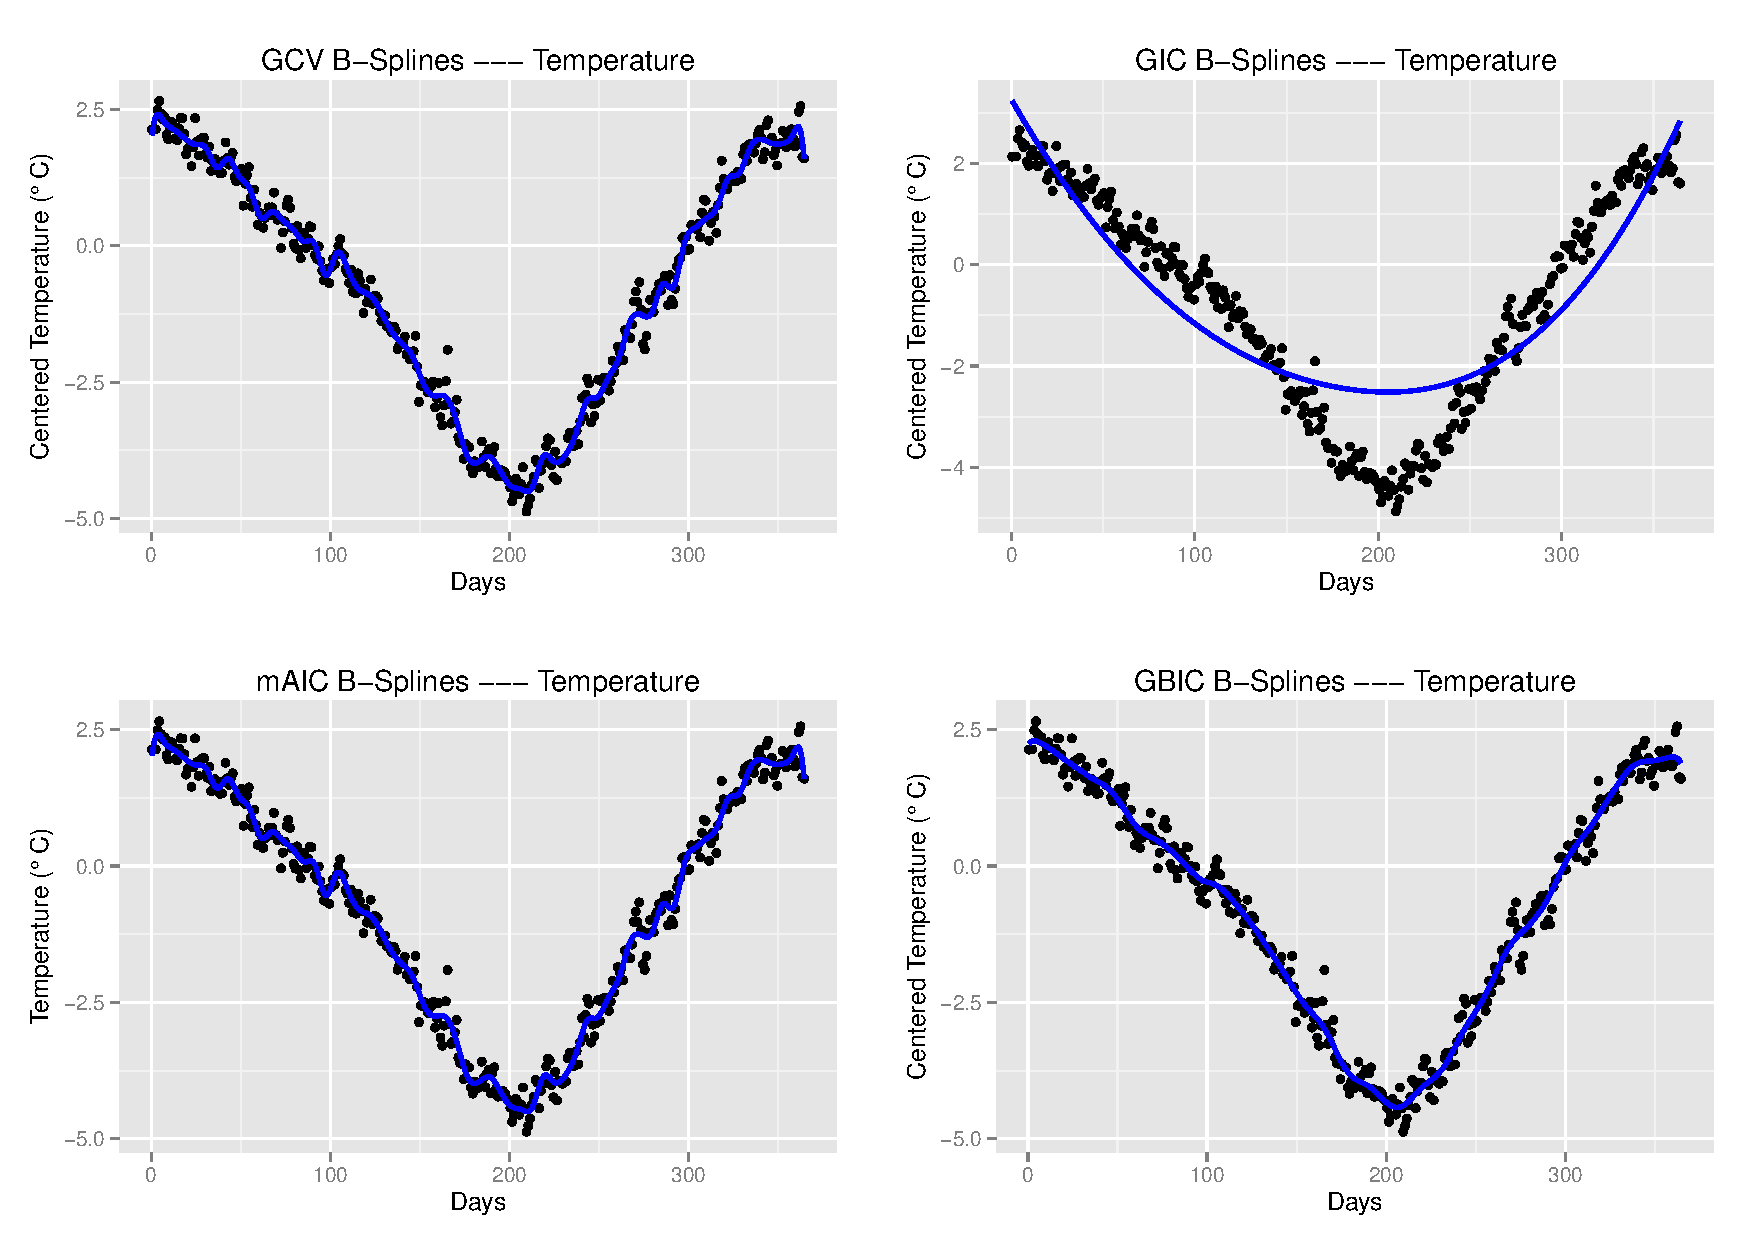
\includegraphics[height=12cm, width=1\textwidth]{Figures/Temp_bsplines_plot.pdf}
  \caption[Fitting Temperature with \textit{Gaussian basis function} on \texttt{A CORUÑA} station]{\textbf{(a)} fitted curve using GCV; \textbf{(b)} fitted curve using GIC; \textbf{(c)} fitted curve using mAIC; \textbf{(d)} fitted curve using GBIC \\ on Temperatures in \texttt{A CORUÑA} }
  \label{fig:Temp_bsplines}
\end{figure}
\clearpage
\subsection{Wind Speed}
Figure~\ref{fig:Wind_bsplines_plot} depicts the fitted curves produced on the observed Wind Speed at \texttt{A CORUÑA} using the information from Table~\ref{table:table_all_stations}. For this case, the \textit{Generalized Information Criterion} and the \textit{Generalized Bayesian Information Criterion} result in small $\hat{K}$ and small $\hat{\lambda}$. The top and bottow right hand side of Figure~\ref{fig:Wind_fourier_plot} show very smooth curves (blue line).

\begin{figure}[th]
  %\centering
    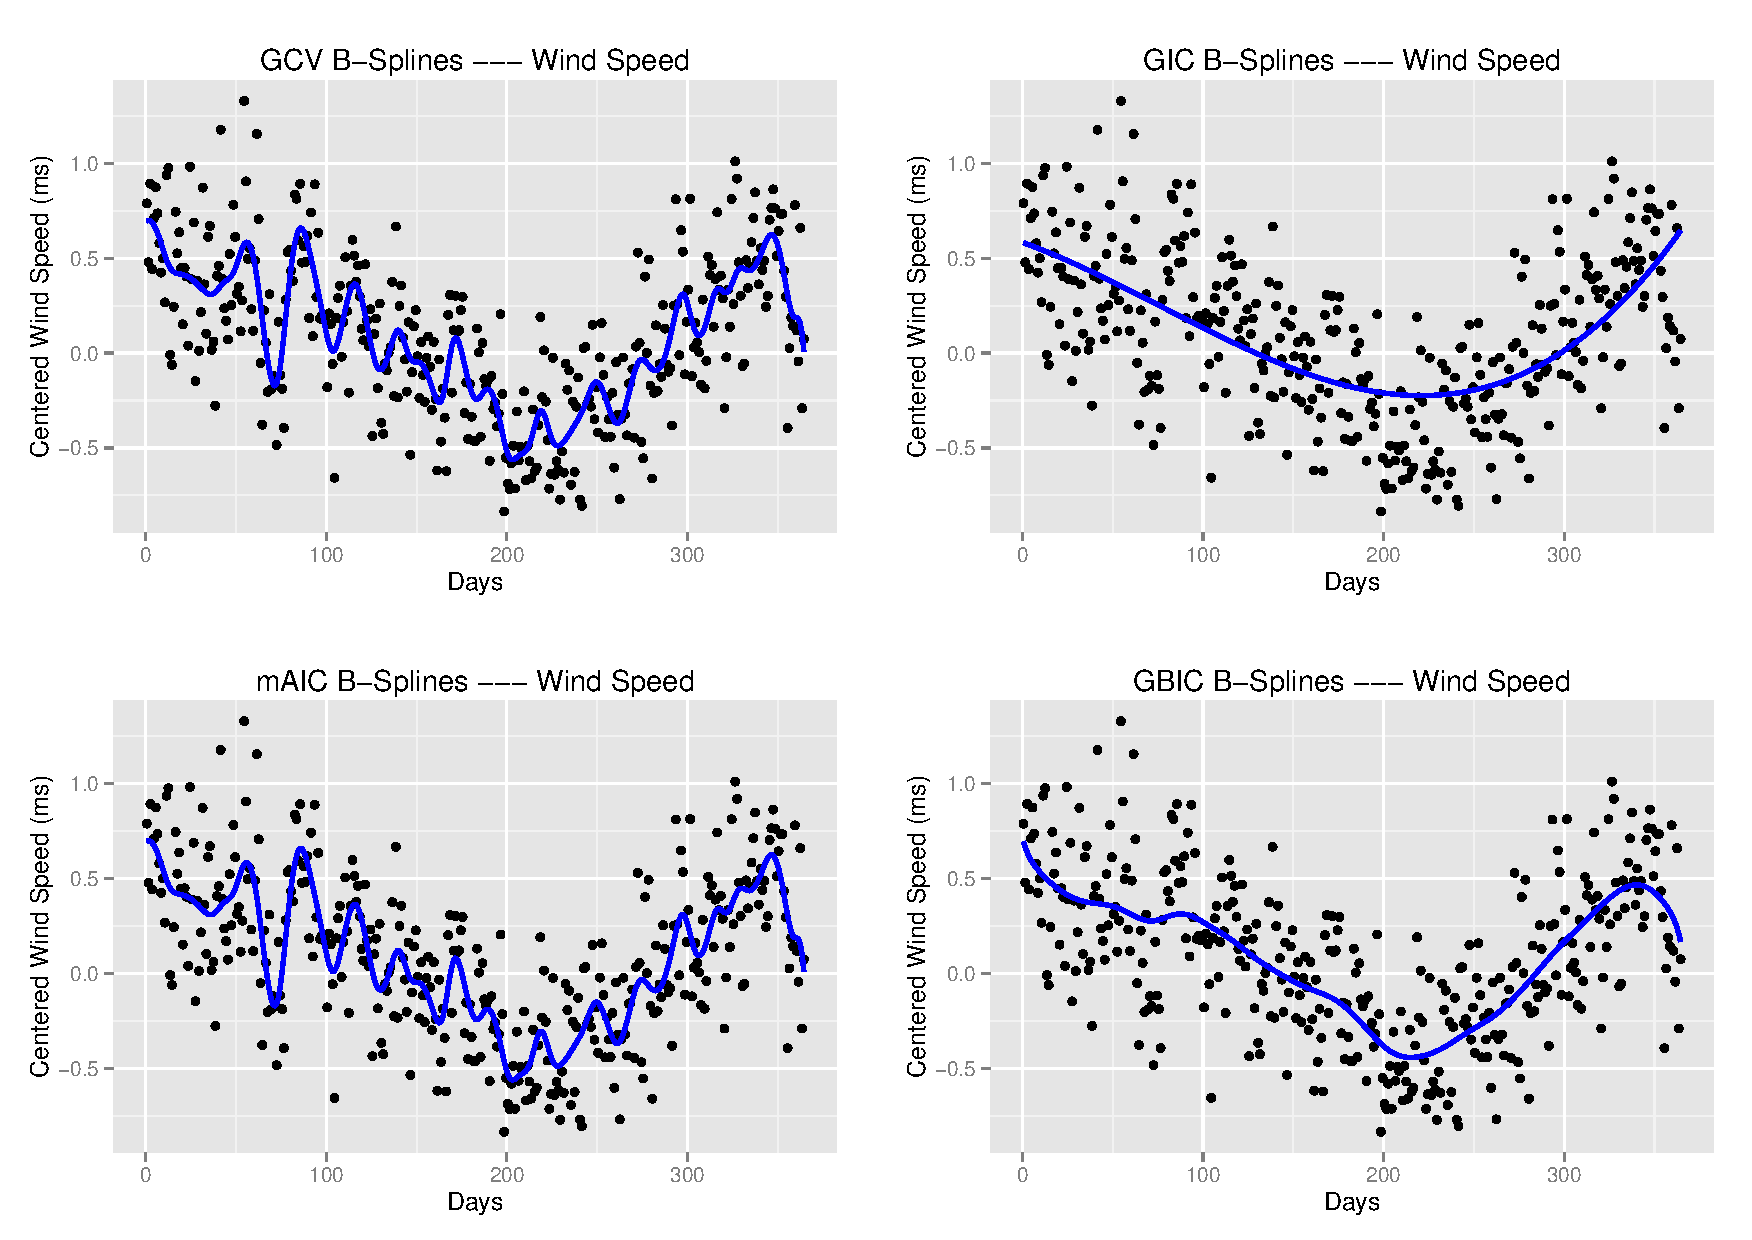
\includegraphics[height=12cm, width=1\textwidth]{Figures/Wind_bsplines_plot.pdf}
  \caption[Fitting Wind Speed with \textit{B-Splines basis function} on \texttt{A CORUÑA} station]{\textbf{(a)} fitted curve using GCV; \textbf{(b)} fitted curve using GIC; \textbf{(c)} fitted curve using mAIC; \textbf{(d)} fitted curve using GBIC \\ on Wind Speed in \texttt{A CORUÑA}}
  \label{fig:Wind_bsplines_plot}
\end{figure}
\subsection{Log-Precipitation}
The computation $\mathbf{\hat{D}}$ and consequently the predicted functional \textit{Log-Precipitation} implies optimizing the matrix of smoothing parameters $\bm{\Lambda}$ for fixed values of $K$ given in Table~\ref{table:table_all_stations}.
\\
Table~\ref{table:summary4} shows the optimal values $\text{log}_{10} (\hat{\lambda}_1)$ and $\text{log}_{10} (\hat{\lambda}_2)$ evaluated for all stations using each model criterion for a fixed the number of basis functions.
\begin{table}[ht]
\caption[Summary of the model selection on the Log-Precipitation using \textit{B-Splines basis functions}]{Summary of the model selection on the Log-Precipitation using \textit{B-Splines basis functions}}
\centering % used for centering table
\begin{tabular}{c @{\hspace{0.2cm}\vrule width 2pt\hspace{0.2cm}} c c c c } % centered columns (4 columns)
\hline %inserts double horizontal lines
\multicolumn{1}{c}{} & & & & \\[-2ex]
 \multicolumn{1}{c}{}& GCV & GIC & mAIC & GBIC \\ [0.5ex] % inserts table
%heading
\noalign{\hrule height 1pt} 
$\text{log}_{10} (\hat{\lambda}_1)$ & -3.51 & -2.15	& -3.72 & -1.33	\\
$\text{log}_{10} (\hat{\lambda}_2)$ & -1.98 & -1.42	& -2.1	& 1.23 \\
$\hat{K}$ & 65 & 5 & 65 & 63 \\
[0.25ex] % [1ex] adds vertical space
\hline  %inserts single line
\end{tabular}
\label{table:summary4} % is used to refer this table in the text
\end{table}

Figure~\ref{fig:logprec_bsplines} depicts the fitted curves produced on the observed Log-Precipitation at \texttt{A CORUÑA} using the information from Table~\ref{table:summary4}. The blue line represents the smooth curve computed using $\bm{D}$ and the red line represents the smooth curve derived from $\bm{\hat{D}}$.

\newpage
\begin{landscape}
\thispagestyle{empty}
\begin{figure}[p]
  \centering
    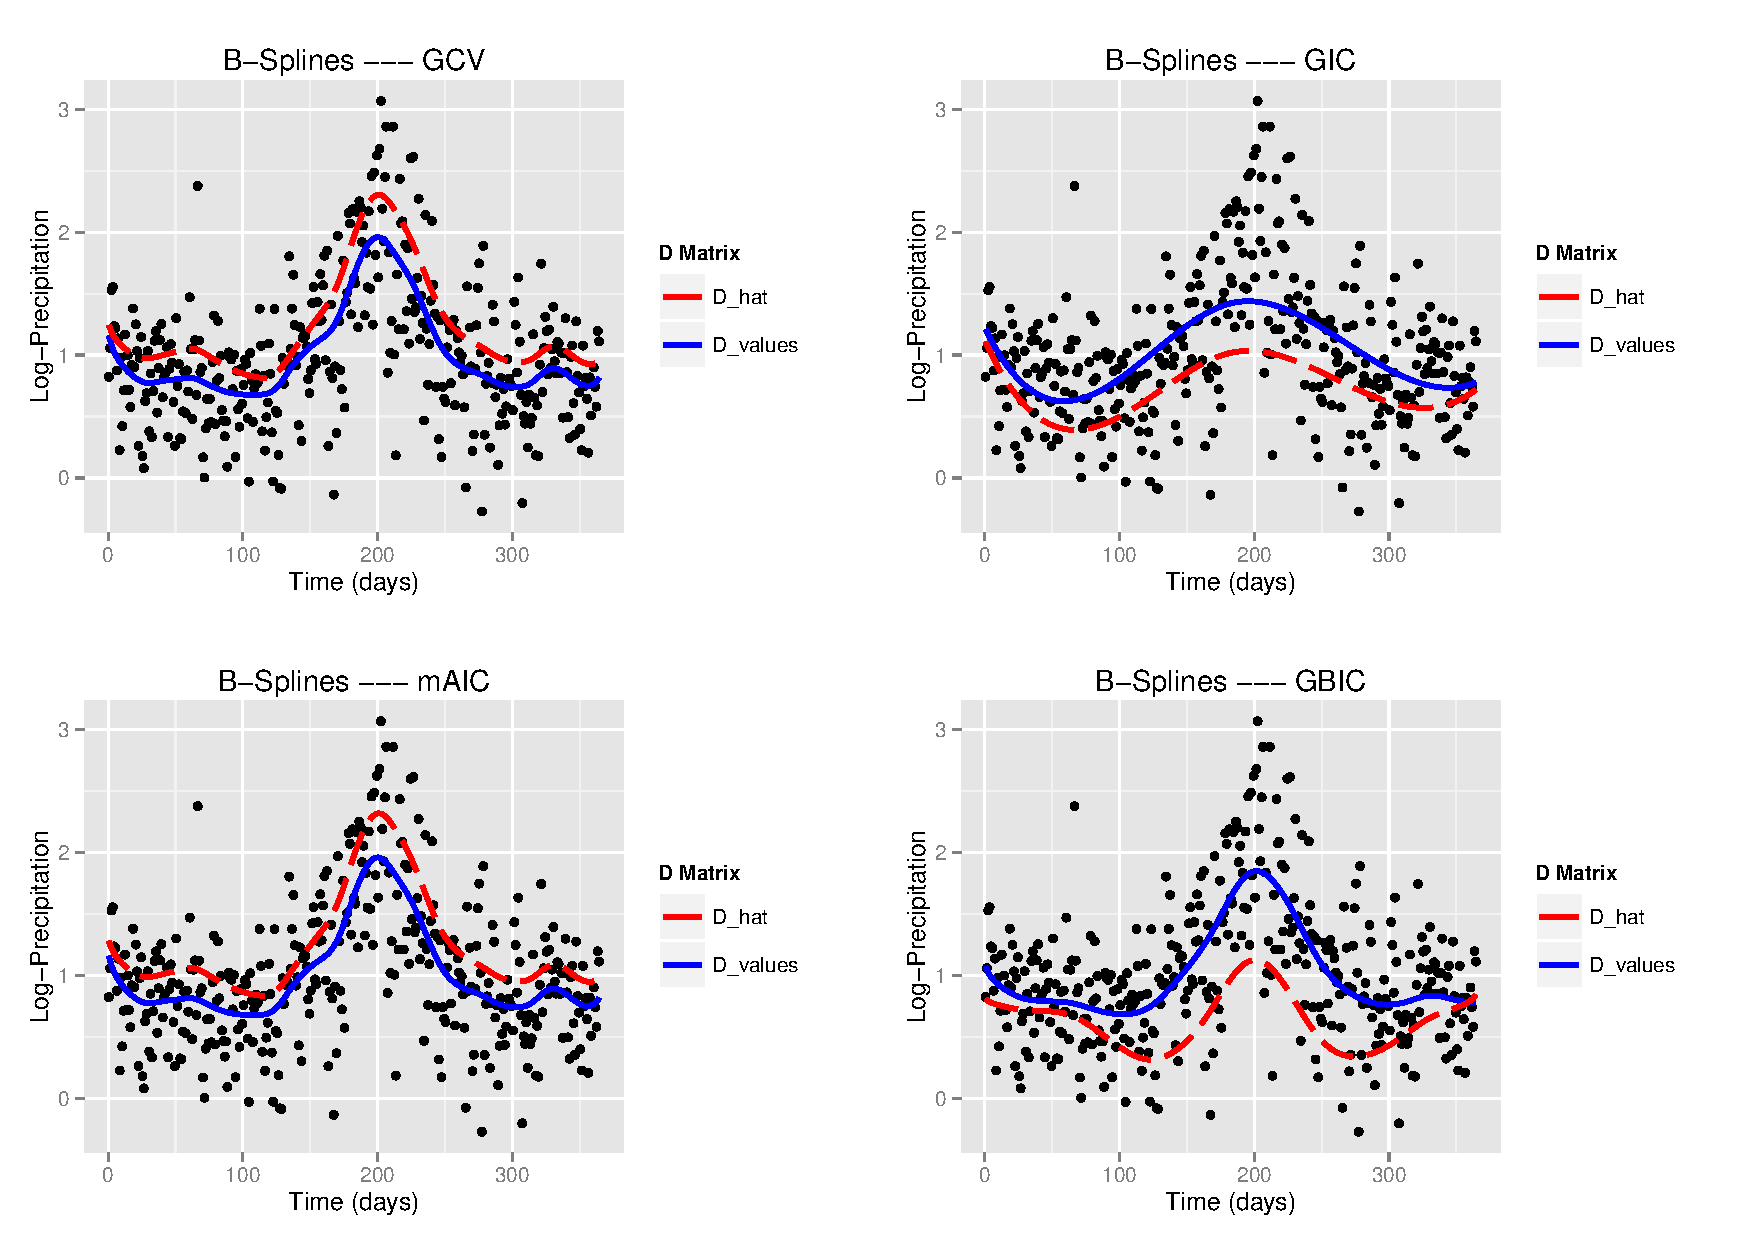
\includegraphics[height=15cm, width=1.7\textwidth]{Figures/D_hat_Bsplines.pdf}
  \caption[Fitting Wind Speed with \textit{Gaussian basis function} on \texttt{A CORUÑA} station]{\textbf{(a)} fitted curve using GCV; \textbf{(b)} fitted curve using GIC; \textbf{(c)} fitted curve using mAIC; \textbf{(d)} fitted curve using GBIC \\ on Log-Precipitation in \texttt{A CORUÑA}}
  \label{fig:logprec_bsplines}
\end{figure}
\end{landscape}   
\newpage

\section{Discussion of the Results}
The objective of this chapter was to illustrate the implementation of a Functional Linear Regression model~\eqref{chap5_eq1} when both covariates and the response variable are functional. The dataset used for illustration was the Spanish weather data. The aim was to model the functional behaviour of the Log-Precipitation when the functional behaviour of the Temperature and Wind Speed were known. The Functional Linear regression Model was computed using the \textit{Penalized Maximum Likelihood} estimate and four model criteria were used to evaluate the model namely: the \textit{Generalized Cross-Validation}; the \textit{Generalized Information Criteria}; the \textit{modified Akaike Information Criteria} and the \textit{Generalized Bayesian Information Criteria}. Three kinds of basis functions were used in the analysis: \textit{Gaussian Basis} function; \textit{Fourier Basis} function and \textit{B-Splines Basis} function. For each kind of basis function and each model criterion, the optimal number of basis functions $\hat{K}$ was estimated as well as the optimal smoothing parameter $\hat{\lambda}$. It was found that, each variable modeled using each kind of basis functions evaluated using each kind model criterion resulted in more or less different values for $\hat{K}$ and the smoothing parameter.
\\
Table~\ref{table:amse} shows the \textit{Mean Square Error} averaged across all stations, for each model criterion and for each type of basis function. In this context, the \textit{Mean Square Error} is defined as the difference between the actual observed data and the predicted: $\bm{\hat{D}} \bm{\Phi}(t)$. Comparing these values across each model criteria is not a very objective way to reach a meaningful conclusion. In fact, it is sensible to compare the results across all types of basis functions.
As given on Table~\ref{table:amse}, the lowest \textit{Average Mean Square Error} (AMSE), considering all models criteria, is found to be at \textit{Gaussian Basis} function. The next type of basis functions is \textit{B-Splines Basis} followed by \textit{Fourier Basis} which appeared to perform the worst out of all three.

\begin{table}[ht]
\caption[\textit{Average Mean Square Error} for the predicted versus observed values of the the functional  \textit{Log-Precipitation}]{\textit{Average Mean Square Error} for the predicted versus observed values of the functional Log-Precipitation} % title of Table
\centering % used for centering table
\begin{tabular}{c c c c} % centered columns (4 columns)
\hline\hline %inserts double horizontal lines
Model Criterion & \textit{Gaussian Basis} & \textit{B-Splines Basis} & \textit{Fourier Basis} \\ [0.5ex] % inserts table
%heading
\hline % inserts single horizontal line
GCV & 0.759 & 0.808 & 0.772 \\ % inserting body of the table
GIC & 1.680 & 1.750 & 2.6 \\
mAIC & 0.759 & 0.791 & 0.772 \\
GBIC & 1.24 & 1.403 & 1.674 \\ [1ex] % [1ex] adds vertical space
\hline %inserts single line
\end{tabular}
\label{table:amse} % is used to refer this table in the text
\end{table}
